% https://tex.stackexchange.com/a/88174/173708
\documentclass[tikz, border=2pt]{standalone}
\usetikzlibrary{mindmap,trees,positioning}
\makeatletter
\tikzset{
    non-concept/.style={
        rectangle,
        text width=12em,
        text=black,
        align=left,
    },
    cncc east/.style={
        edge from parent path={
            (\tikzparentnode.east) to[out=0, in=180] (\tikzchildnode.south west)
            -- (\tikzchildnode.south east)
        }
    }
}
\makeatother
\begin{document}
\pagestyle{empty}
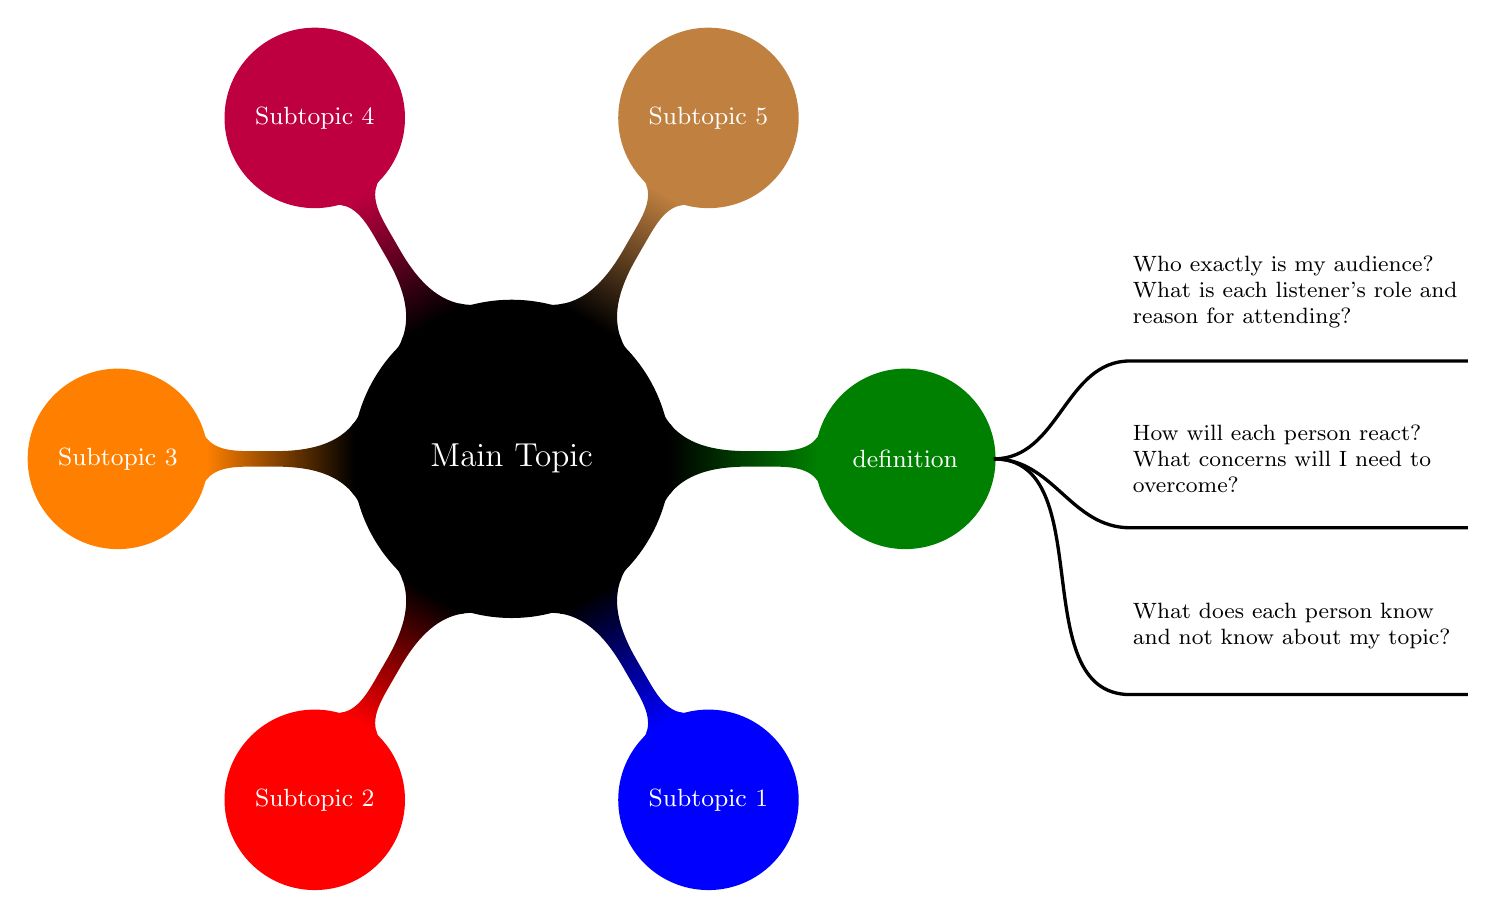
\begin{tikzpicture}
  \path[mindmap, concept color=black, text=white]
    node[concept] {Main Topic}[clockwise from=0]% named \___/ node
    child[concept color=green!50!black] {
        node[concept] (def) {definition}
        [
            grow=right,
            sibling distance=14ex,
        ]
            child[level distance=5cm] 
            	{ node[non-concept] 
            		{What does each person know and not know about my topic?}                            
            	edge from parent[cncc east] }
		child[level distance=5cm] 
			{ node[non-concept] 
				{How will each person react? What concerns will I need to overcome?}                 
			edge from parent[cncc east] }
		child[level distance=5cm] 
			{ node[non-concept] 
				{Who exactly is my audience? What is each listener's role and reason for attending?} 
			edge from parent[cncc east] }
        }
    child[concept color=blue]           { node[concept]       {Subtopic 1} }
    child[concept color=red]            { node[concept]       {Subtopic 2} }
    child[concept color=orange]         { node[concept]       {Subtopic 3} }
    child[concept color=purple]         { node[concept]       {Subtopic 4} }
    child[concept color=brown]          { node[concept]       {Subtopic 5} };
\end{tikzpicture}
\end{document}